\RequirePackage{atbegshi}
\documentclass[compress,aspectratio=169]{beamer}\usepackage[]{graphicx}\usepackage[]{color}
%% maxwidth is the original width if it is less than linewidth
%% otherwise use linewidth (to make sure the graphics do not exceed the margin)
\makeatletter
\def\maxwidth{ %
  \ifdim\Gin@nat@width>\linewidth
    \linewidth
  \else
    \Gin@nat@width
  \fi
}
\makeatother

\definecolor{fgcolor}{rgb}{0.345, 0.345, 0.345}
\newcommand{\hlnum}[1]{\textcolor[rgb]{0.686,0.059,0.569}{#1}}%
\newcommand{\hlstr}[1]{\textcolor[rgb]{0.192,0.494,0.8}{#1}}%
\newcommand{\hlcom}[1]{\textcolor[rgb]{0.678,0.584,0.686}{\textit{#1}}}%
\newcommand{\hlopt}[1]{\textcolor[rgb]{0,0,0}{#1}}%
\newcommand{\hlstd}[1]{\textcolor[rgb]{0.345,0.345,0.345}{#1}}%
\newcommand{\hlkwa}[1]{\textcolor[rgb]{0.161,0.373,0.58}{\textbf{#1}}}%
\newcommand{\hlkwb}[1]{\textcolor[rgb]{0.69,0.353,0.396}{#1}}%
\newcommand{\hlkwc}[1]{\textcolor[rgb]{0.333,0.667,0.333}{#1}}%
\newcommand{\hlkwd}[1]{\textcolor[rgb]{0.737,0.353,0.396}{\textbf{#1}}}%
\let\hlipl\hlkwb

\usepackage{framed}
\makeatletter
\newenvironment{kframe}{%
 \def\at@end@of@kframe{}%
 \ifinner\ifhmode%
  \def\at@end@of@kframe{\end{minipage}}%
  \begin{minipage}{\columnwidth}%
 \fi\fi%
 \def\FrameCommand##1{\hskip\@totalleftmargin \hskip-\fboxsep
 \colorbox{shadecolor}{##1}\hskip-\fboxsep
     % There is no \\@totalrightmargin, so:
     \hskip-\linewidth \hskip-\@totalleftmargin \hskip\columnwidth}%
 \MakeFramed {\advance\hsize-\width
   \@totalleftmargin\z@ \linewidth\hsize
   \@setminipage}}%
 {\par\unskip\endMakeFramed%
 \at@end@of@kframe}
\makeatother

\definecolor{shadecolor}{rgb}{.97, .97, .97}
\definecolor{messagecolor}{rgb}{0, 0, 0}
\definecolor{warningcolor}{rgb}{1, 0, 1}
\definecolor{errorcolor}{rgb}{1, 0, 0}
\newenvironment{knitrout}{}{} % an empty environment to be redefined in TeX

\usepackage{alltt} % aspectratio=169
%\usepackage[svgnames]{xcolor}

% % % % % % % % % % % % % % %
%             MY PACKAGES 
% % % % % % % % % % % % % % %
\usepackage{graphicx}       % Use pdf, png, jpg, or eps with pdflatex; use eps in DVI mode
\usepackage{dcolumn} % this pack is neccesary to build nicer columns with texreg--dont remove it.
\usepackage[export]{adjustbox}
\usepackage{amssymb}
\usepackage{amsmath}  
%\usepackage{tipx}
%\usepackage{tikz}
%\usetikzlibrary{arrows,shapes,decorations.pathmorphing,backgrounds,positioning,fit,petri}
\usepackage{rotating}
%\usepackage{scalerel} % for inline images
\usepackage{import}
%\usepackage{times}
\usepackage{array}
\usepackage{tabularx}
%\usepackage{booktabs}
%\usepackage{textcomp}
\usepackage{float}
%\usepackage{setspace}      % \doublespacing \singlespacing \onehalfspacing %doble espacio
%\label{x:y}                          %ocupar para autoref.
%\autoref{x:y}                        %ocupar para autoref.
%\usepackage{nopageno}      %desactivar para p<U+FFFD><U+FFFD><U+FFFD>ginas
\usepackage{pifont}
%\usepackage{color,xcolor,ucs}
%\usepackage{marvosym} %faces
\usepackage{hyperref}
\usepackage{multirow}


\usepackage{listings}
\usepackage{color}
\definecolor{dkgreen}{rgb}{0,0.6,0}
\definecolor{gray}{rgb}{0.5,0.5,0.5}
\definecolor{mauve}{rgb}{0.58,0,0.82}
\lstset{ %
  language=R,                     % the language of the code
  basicstyle=\TINY,           % the size of the fonts that are used for the code
  numbers=left,                   % where to put the line-numbers
  numberstyle=\tiny\color{gray},  % the style that is used for the line-numbers
  stepnumber=1,                   % the step between two line-numbers. If it's 1, each line
                                  % will be numbered
  numbersep=5pt,                  % how far the line-numbers are from the code
  backgroundcolor=\color{white},  % choose the background color. You must add \usepackage{color}
  showspaces=false,               % show spaces adding particular underscores
  showstringspaces=false,         % underline spaces within strings
  showtabs=false,                 % show tabs within strings adding particular underscores
  frame=single,                   % adds a frame around the code
  rulecolor=\color{black},        % if not set, the frame-color may be changed on line-breaks within not-black text (e.g. commens (green here))
  tabsize=1,                      % sets default tabsize to 2 spaces
  captionpos=b,                   % sets the caption-position to bottom
  breaklines=true,                % sets automatic line breaking
  breakatwhitespace=false,        % sets if automatic breaks should only happen at whitespace
  title=\lstname,                 % show the filename of files included with \lstinputlisting;
                                  % also try caption instead of title
  keywordstyle=\color{blue},      % keyword style
  commentstyle=\color{dkgreen},   % comment style
  stringstyle=\color{mauve},      % string literal style
  escapeinside={\%*}{*)},         % if you want to add a comment within your code
  morekeywords={*,...}            % if you want to add more keywords to the set
} 

% % % % % % % % % % % % % % %
%           PACKAGE CUSTOMIZATION
% % % % % % % % % % % % % % %

% GENERAL CUSTOMIZATION
\usepackage[math]{iwona}% font
\usetheme{Singapore}  % template I should use
%\usetheme{Szeged}  % alternative template
\usecolortheme{rose}  % color template
\makeatletter     % to show subsection/section title (1/3)
\beamer@theme@subsectiontrue % to show subsection/section title (2/3)
\makeatother      % to show subsection/section title (3/3)



% THIS BELOW IS TO MAKE NAVIGATION DOTS MARKED DURING PRESENTATION
\makeatletter
\def\slideentry#1#2#3#4#5#6{%
  %section number, subsection number, slide number, first/last frame, page number, part number
  \ifnum#6=\c@part\ifnum#2>0\ifnum#3>0%
    \ifbeamer@compress%
      \advance\beamer@xpos by1\relax%
    \else%
      \beamer@xpos=#3\relax%
      \beamer@ypos=#2\relax%
    \fi%
  \hbox to 0pt{%
    \beamer@tempdim=-\beamer@vboxoffset%
    \advance\beamer@tempdim by-\beamer@boxsize%
    \multiply\beamer@tempdim by\beamer@ypos%
    \advance\beamer@tempdim by -.05cm%
    \raise\beamer@tempdim\hbox{%
      \beamer@tempdim=\beamer@boxsize%
      \multiply\beamer@tempdim by\beamer@xpos%
      \advance\beamer@tempdim by -\beamer@boxsize%
      \advance\beamer@tempdim by 1pt%
      \kern\beamer@tempdim
      \global\beamer@section@min@dim\beamer@tempdim
      \hbox{\beamer@link(#4){%
          \usebeamerfont{mini frame}%
          \ifnum\c@section>#1%
            %\usebeamercolor[fg]{mini frame}%
            %\usebeamertemplate{mini frame}%
            \usebeamercolor{mini frame}%
            \usebeamertemplate{mini frame in other subsection}%
          \else%
            \ifnum\c@section=#1%
              \ifnum\c@subsection>#2%
                \usebeamercolor[fg]{mini frame}%
                \usebeamertemplate{mini frame}%
              \else%
                \ifnum\c@subsection=#2%
                  \usebeamercolor[fg]{mini frame}%
                  \ifnum\c@subsectionslide<#3%
                    \usebeamertemplate{mini frame in current subsection}%
                  \else%
                    \usebeamertemplate{mini frame}%
                  \fi%
                \else%
                  \usebeamercolor{mini frame}%
                  \usebeamertemplate{mini frame in other subsection}%
                \fi%
              \fi%
            \else%
              \usebeamercolor{mini frame}%
              \usebeamertemplate{mini frame in other subsection}%
            \fi%
          \fi%
        }}}\hskip-10cm plus 1fil%
  }\fi\fi%
  \else%
  \fakeslideentry{#1}{#2}{#3}{#4}{#5}{#6}%
  \fi\ignorespaces
  }
\makeatother


% % % % % % % % % % % % % % %
%       To show the TITLE at the Bottom of each slide
% % % % % % % % % % % % % % %

\beamertemplatenavigationsymbolsempty 
\makeatletter
\setbeamertemplate{footline}
{
\leavevmode%
\hbox{%
\begin{beamercolorbox}[wd=1\paperwidth,ht=2.25ex,dp=2ex,center]{title in head/foot}%
\usebeamerfont{title in head/foot}\insertshorttitle
\end{beamercolorbox}%
\begin{beamercolorbox}[wd=1
\paperwidth,ht=2.25ex,dp=2ex,center]{date in head/foot}%
\end{beamercolorbox}}%
}
\makeatother



% to switch off navigation bullets
%% using \miniframeson or \miniframesoff
\makeatletter
\let\beamer@writeslidentry@miniframeson=\beamer@writeslidentry
\def\beamer@writeslidentry@miniframesoff{%
  \expandafter\beamer@ifempty\expandafter{\beamer@framestartpage}{}% does not happen normally
  {%else
    % removed \addtocontents commands
    \clearpage\beamer@notesactions%
  }
}
\newcommand*{\miniframeson}{\let\beamer@writeslidentry=\beamer@writeslidentry@miniframeson}
\newcommand*{\miniframesoff}{\let\beamer@writeslidentry=\beamer@writeslidentry@miniframesoff}
\makeatother

% Image full size: use 
%%\begin{frame}
  %%\fullsizegraphic{monogram.jpg}
%%\end{frame}
\newcommand<>{\fullsizegraphic}[1]{
  \begin{textblock*}{0cm}(-1cm,-3.78cm)
  \includegraphics[width=\paperwidth]{#1}
  \end{textblock*}
}


% hyperlinks
\hypersetup{colorlinks,
            urlcolor=[rgb]{0.01, 0.28, 1.0},
            linkcolor=[rgb]{0.01, 0.28, 1.0}}


% % % % % % % % % % % % % % %
%           DOCUMENT ID
% % % % % % % % % % % % % % %

\title{\href{https://doi.org/10.1057/s41269-020-00174-4}{\input{/Users/hectorbahamonde/research/Vote_Selling/title.txt}\unskip}}



\author[shortname]{H\'ector Bahamonde}
\institute[shortinst]{Assistant Professor, O$'$Higgins University (Chile)}
\date{\today}

%to to see shadows of previous blocks
%\setbeamercovered{dynamic}
\IfFileExists{upquote.sty}{\usepackage{upquote}}{}
\begin{document}



% % % % % % % % % % % % % % %
%           CONTENT
% % % % % % % % % % % % % % %

%% title frame

\begin{frame}[label = cover]
\titlepage
\end{frame}




\section{Introduction}

\subsection{Introduction}

\miniframeson
\begin{frame}\frametitle{{\scriptsize ``{\input{/Users/hectorbahamonde/research/Vote_Selling/title.txt}\unskip}'' }}
\begin{minipage}{0.47\textwidth}
    \begin{itemize}
          \item \emph{Acta Politica} (WOS), 2020.
          \item Under review since June 2019, and accepted for publication in July 2020.
          \item About: clientelism; vote buying.
    \end{itemize}
\end{minipage}
\begin{minipage}{0.5\textwidth}
\centering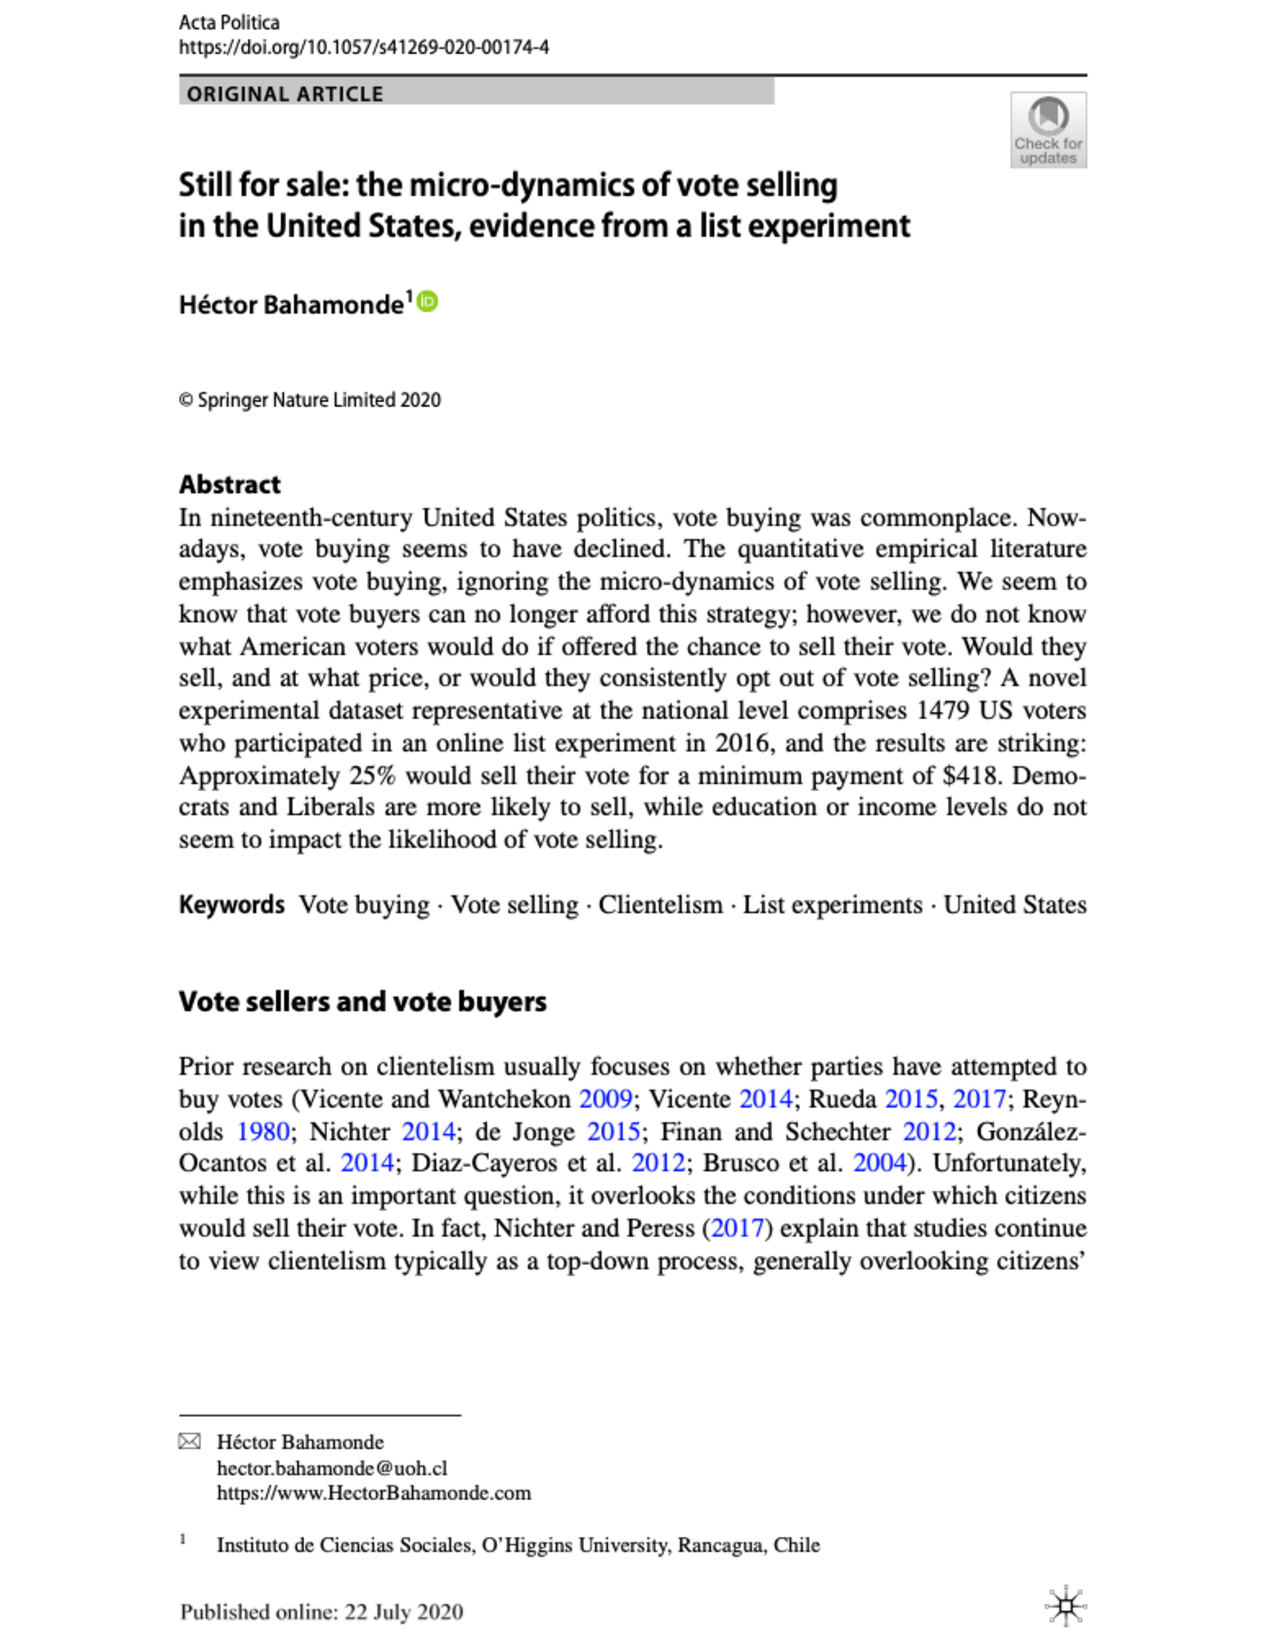
\includegraphics[scale=0.2]{/Users/hectorbahamonde/research/Vote_Selling/Journal_Cover.pdf}
\end{minipage}
\end{frame}



\miniframeson
\begin{frame}\frametitle{Summary}
        \begin{itemize}
          \item Using a least-likely case design (U.S.), the paper studies voter's willingness to sell their vote in exchange for money.
          \item Data are novel and are representative at the country level (N = 1,479).
          \item List experiment (survey experiment).\pause
          \item Findings:
            \begin{enumerate}
              \item Approximately 25\% of voters in the U.S. would sell their vote.
              \item They would sell it for a minimum payment of \$418. 
              \item Democrats and Liberals are more likely to sell.
              \item Education or income levels do not seem to impact the likelihood of vote selling.
              \end{enumerate}
        \end{itemize}
\end{frame}


\section{Motivation}
\subsection{Motivation}

\miniframeson
\begin{frame}\frametitle{Wrong Impressions: From \emph{Did} you to \emph{Would} you}
\begin{minipage}{0.47\textwidth}
    \begin{itemize}
          \item Americans have rarely been offered the chance to sell their vote.
          \item However, the question stands: \emph{Would they?}
          \item {\bf Does this question matter?} {\color{white}It \emph{does}: the figure it gives the wrong impression that US voters systematically ``oppose'' vote buying, ``thus'' rarely engaging in it.}
    \end{itemize}
\end{minipage}
\begin{minipage}{0.5\textwidth}
\centering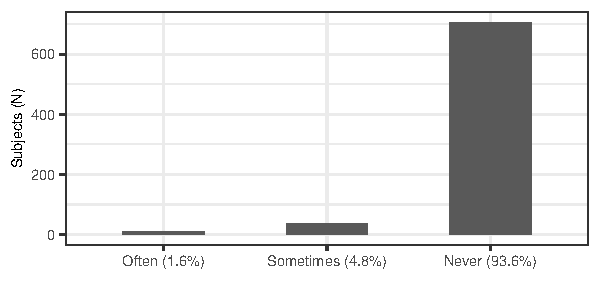
\includegraphics[scale=0.75]{/Users/hectorbahamonde/research/Vote_Selling/figure/lapop:bar:chart:plot-1.pdf}
{\tiny Source: LAPOP 2010.}
\end{minipage}
\end{frame}

\miniframesoff
\begin{frame}\frametitle{Wrong Impressions: From \emph{Did} you to \emph{Would} you}
\begin{minipage}{0.47\textwidth}
    \begin{itemize}
          \item Americans have rarely been offered the chance to sell their vote.
          \item However, the question stands: \emph{Would they?}
          \item {\bf Does this question matter?} It \emph{does}: the figure it gives the wrong impression that US voters systematically ``oppose'' vote buying, ``thus'' rarely engaging in it.
    \end{itemize}
\end{minipage}
\begin{minipage}{0.5\textwidth}
\centering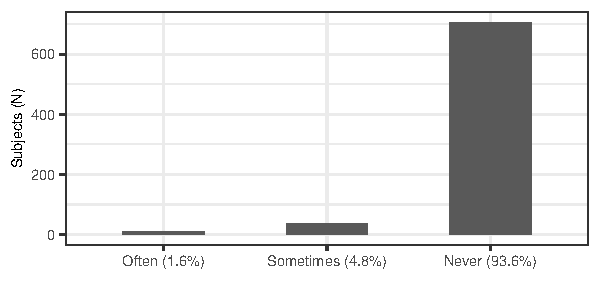
\includegraphics[scale=0.75]{/Users/hectorbahamonde/research/Vote_Selling/figure/lapop:bar:chart:plot-1.pdf}
{\tiny Source: LAPOP 2010.}
\end{minipage}
\end{frame}

\miniframeson
\begin{frame}\frametitle{Literature Suffers from Selection Bias}
    \begin{itemize}
          \item Clientelism literature has focused on realized transactions only: developing countries.
          \item Unfortunately, studying only cases where the outcome of interest is produced, causes selection bias {\tiny (Geddes, 1990)}.
            \begin{itemize}
              \item Studying actual behaviors only limits both the questions and causal inferences.
            \end{itemize}
          \item My paper fills these gaps by studying hypothetical behaviors (willingness to sell) in a developed country: U.S.\\{\bf ``Least-likely case design.''}
    \end{itemize}
\end{frame}



\section{The U.S. as a Case}


\subsection{History}

\miniframeson
\begin{frame}\frametitle{Vote Buying Was Very Common in the U.S.}
\begin{minipage}{0.7\textwidth}
    \begin{itemize}
          \item George Washington spent 40 pounds (a considerable sum for the day) on gallons of rum, wine, brandy, and beer; all used to buy votes.
          \item Party tickets.
          \item Institutions: the \emph{viva voce} and \emph{Australian ballot} methods.
    \end{itemize}
\end{minipage}
\begin{minipage}{0.1\textwidth}
\centering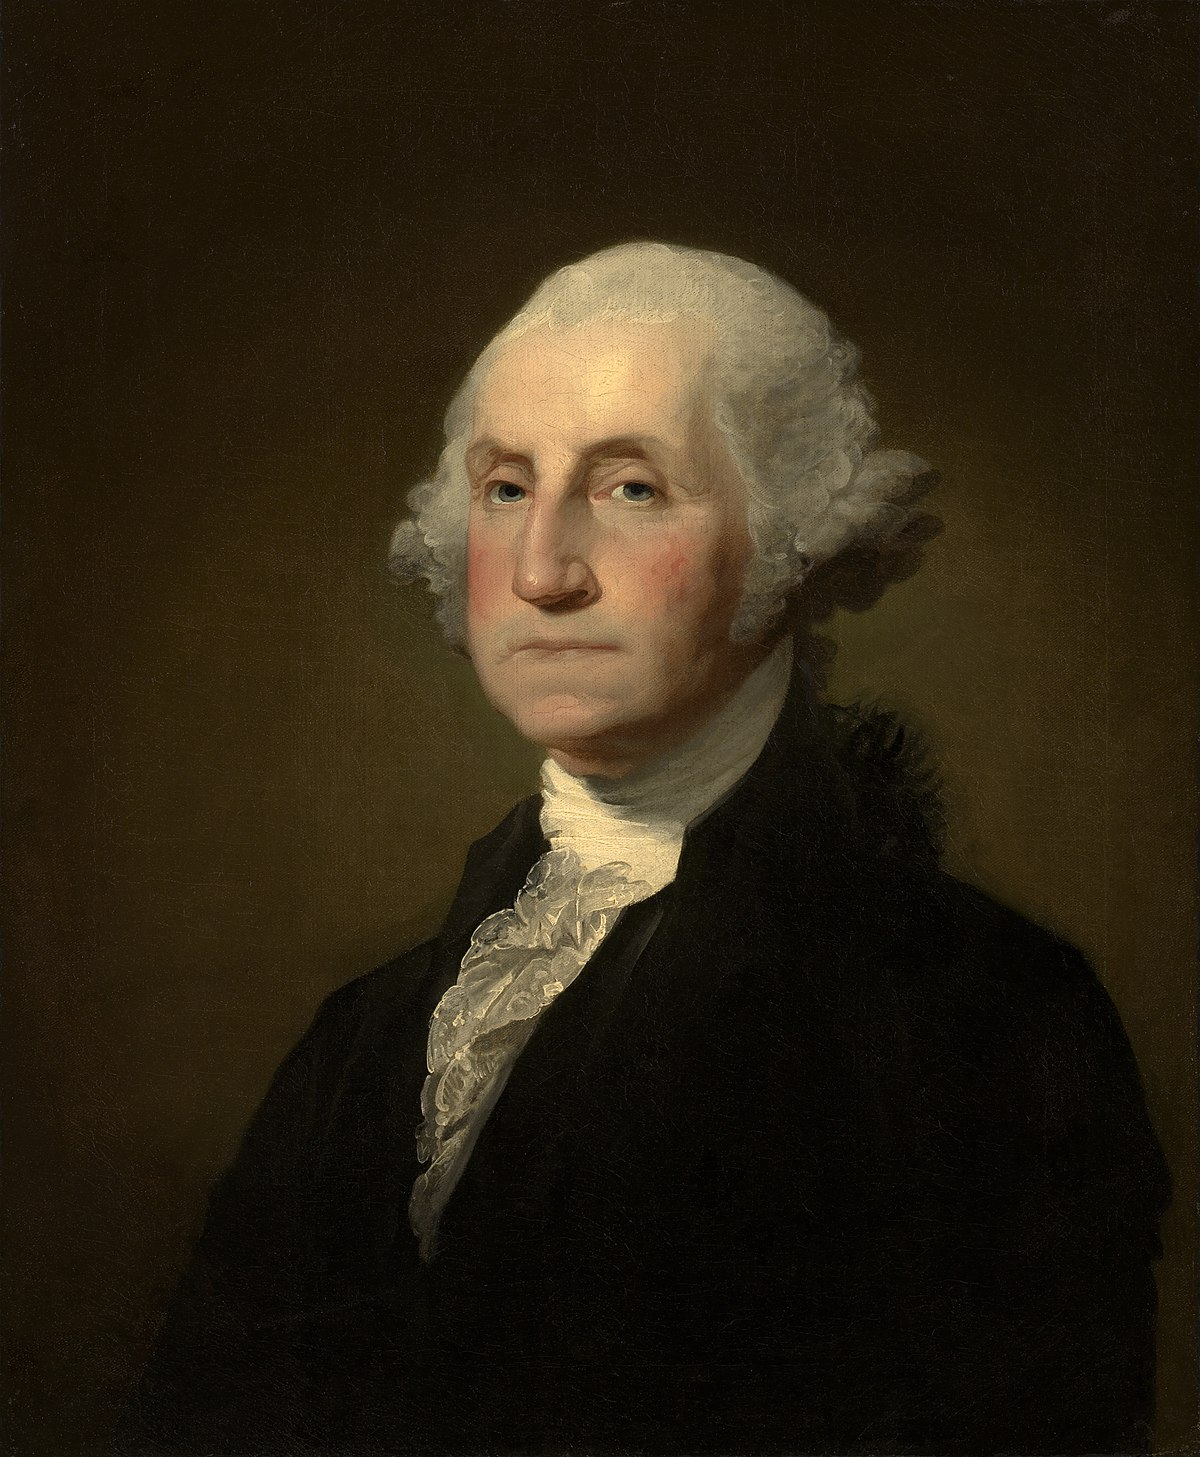
\includegraphics[scale=0.09]{/Users/hectorbahamonde/research/Vote_Selling/george_washington.jpg}
\end{minipage}
\end{frame}


\miniframeson
\begin{frame}\frametitle{Now Vote Buying is Rare}
    \begin{itemize}
          \item Two competing hypotheses:
            \begin{enumerate}
              \item {\bf Kitschelt}: shrinkage of the state.
              \item {\bf Stokes}: industrialization drove up the electorate's median income, making vote buying more expensive for party machines.\pause
            \end{enumerate}
            \item My paper does \emph{not} test nor does it explore the causes of decayed clientelism in the U.S.
    \end{itemize}
\end{frame}



\section{Empirical Section}

\subsection{Research Question and Data}

\miniframeson
\begin{frame}%\frametitle{Setup}
\begin{minipage}{0.4\textwidth}
    \begin{itemize}
          \item {\bf Research Question}: \emph{What is the willingness to sell of American voters when offered the chance to sell their votes?}
          \item {\bf Data}: Online panel (N=1,479) representative at the country level. {\scriptsize Re-sampling of gender and party ID}.
    \end{itemize}
\end{minipage}
\begin{minipage}{0.5\textwidth}
\centering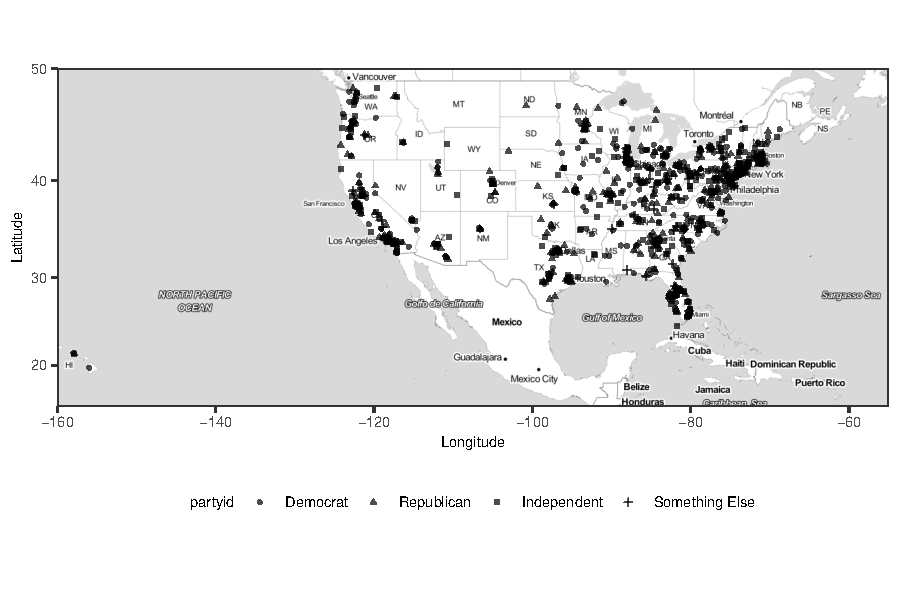
\includegraphics[scale=0.6]{/Users/hectorbahamonde/research/Vote_Selling/figure/us:map:plot-1.pdf}
\end{minipage}
\end{frame}



\subsection{Methods}

\miniframeson
\begin{frame}\frametitle{The Study of Vote Selling Introduces Social Desirability Bias}
    \begin{itemize}
      \item Directly asking respondents whether they would sell their votes will cause {\bf social desirability bias}.
      \item Respondents might feel ashamed admitting doing something socially condemnable.
    \end{itemize}
\end{frame}


\miniframeson
\begin{frame}\frametitle{The Use of List Experiments Overcomes Social Desirability Bias}
    \begin{itemize}
      \item {\bf List experiments} designed to study illegal/uncommon behaviors (drug consumption, corruption, sexual behaviors).
      \item {\bf Mechanics}: 
        \begin{itemize}
            \item Two lists (control, treatment). Both are \emph{exactly} the same. 
            \item The treatment has an extra item, the {\bf sensitive} one.
            \item {\bf Respondent's task}: declare how many items (not which ones) s/he would endorse.
        \end{itemize}
      \item {\bf Easy estimation}: since both lists are assigned at random, any difference in means between the {\bf item count} of the treatment and control lists should be attributed to the sensitive item \emph{only}.
    \end{itemize}
\end{frame}


\miniframesoff
\begin{frame}[plain]
 %\vspace{-0.5cm}
  \centering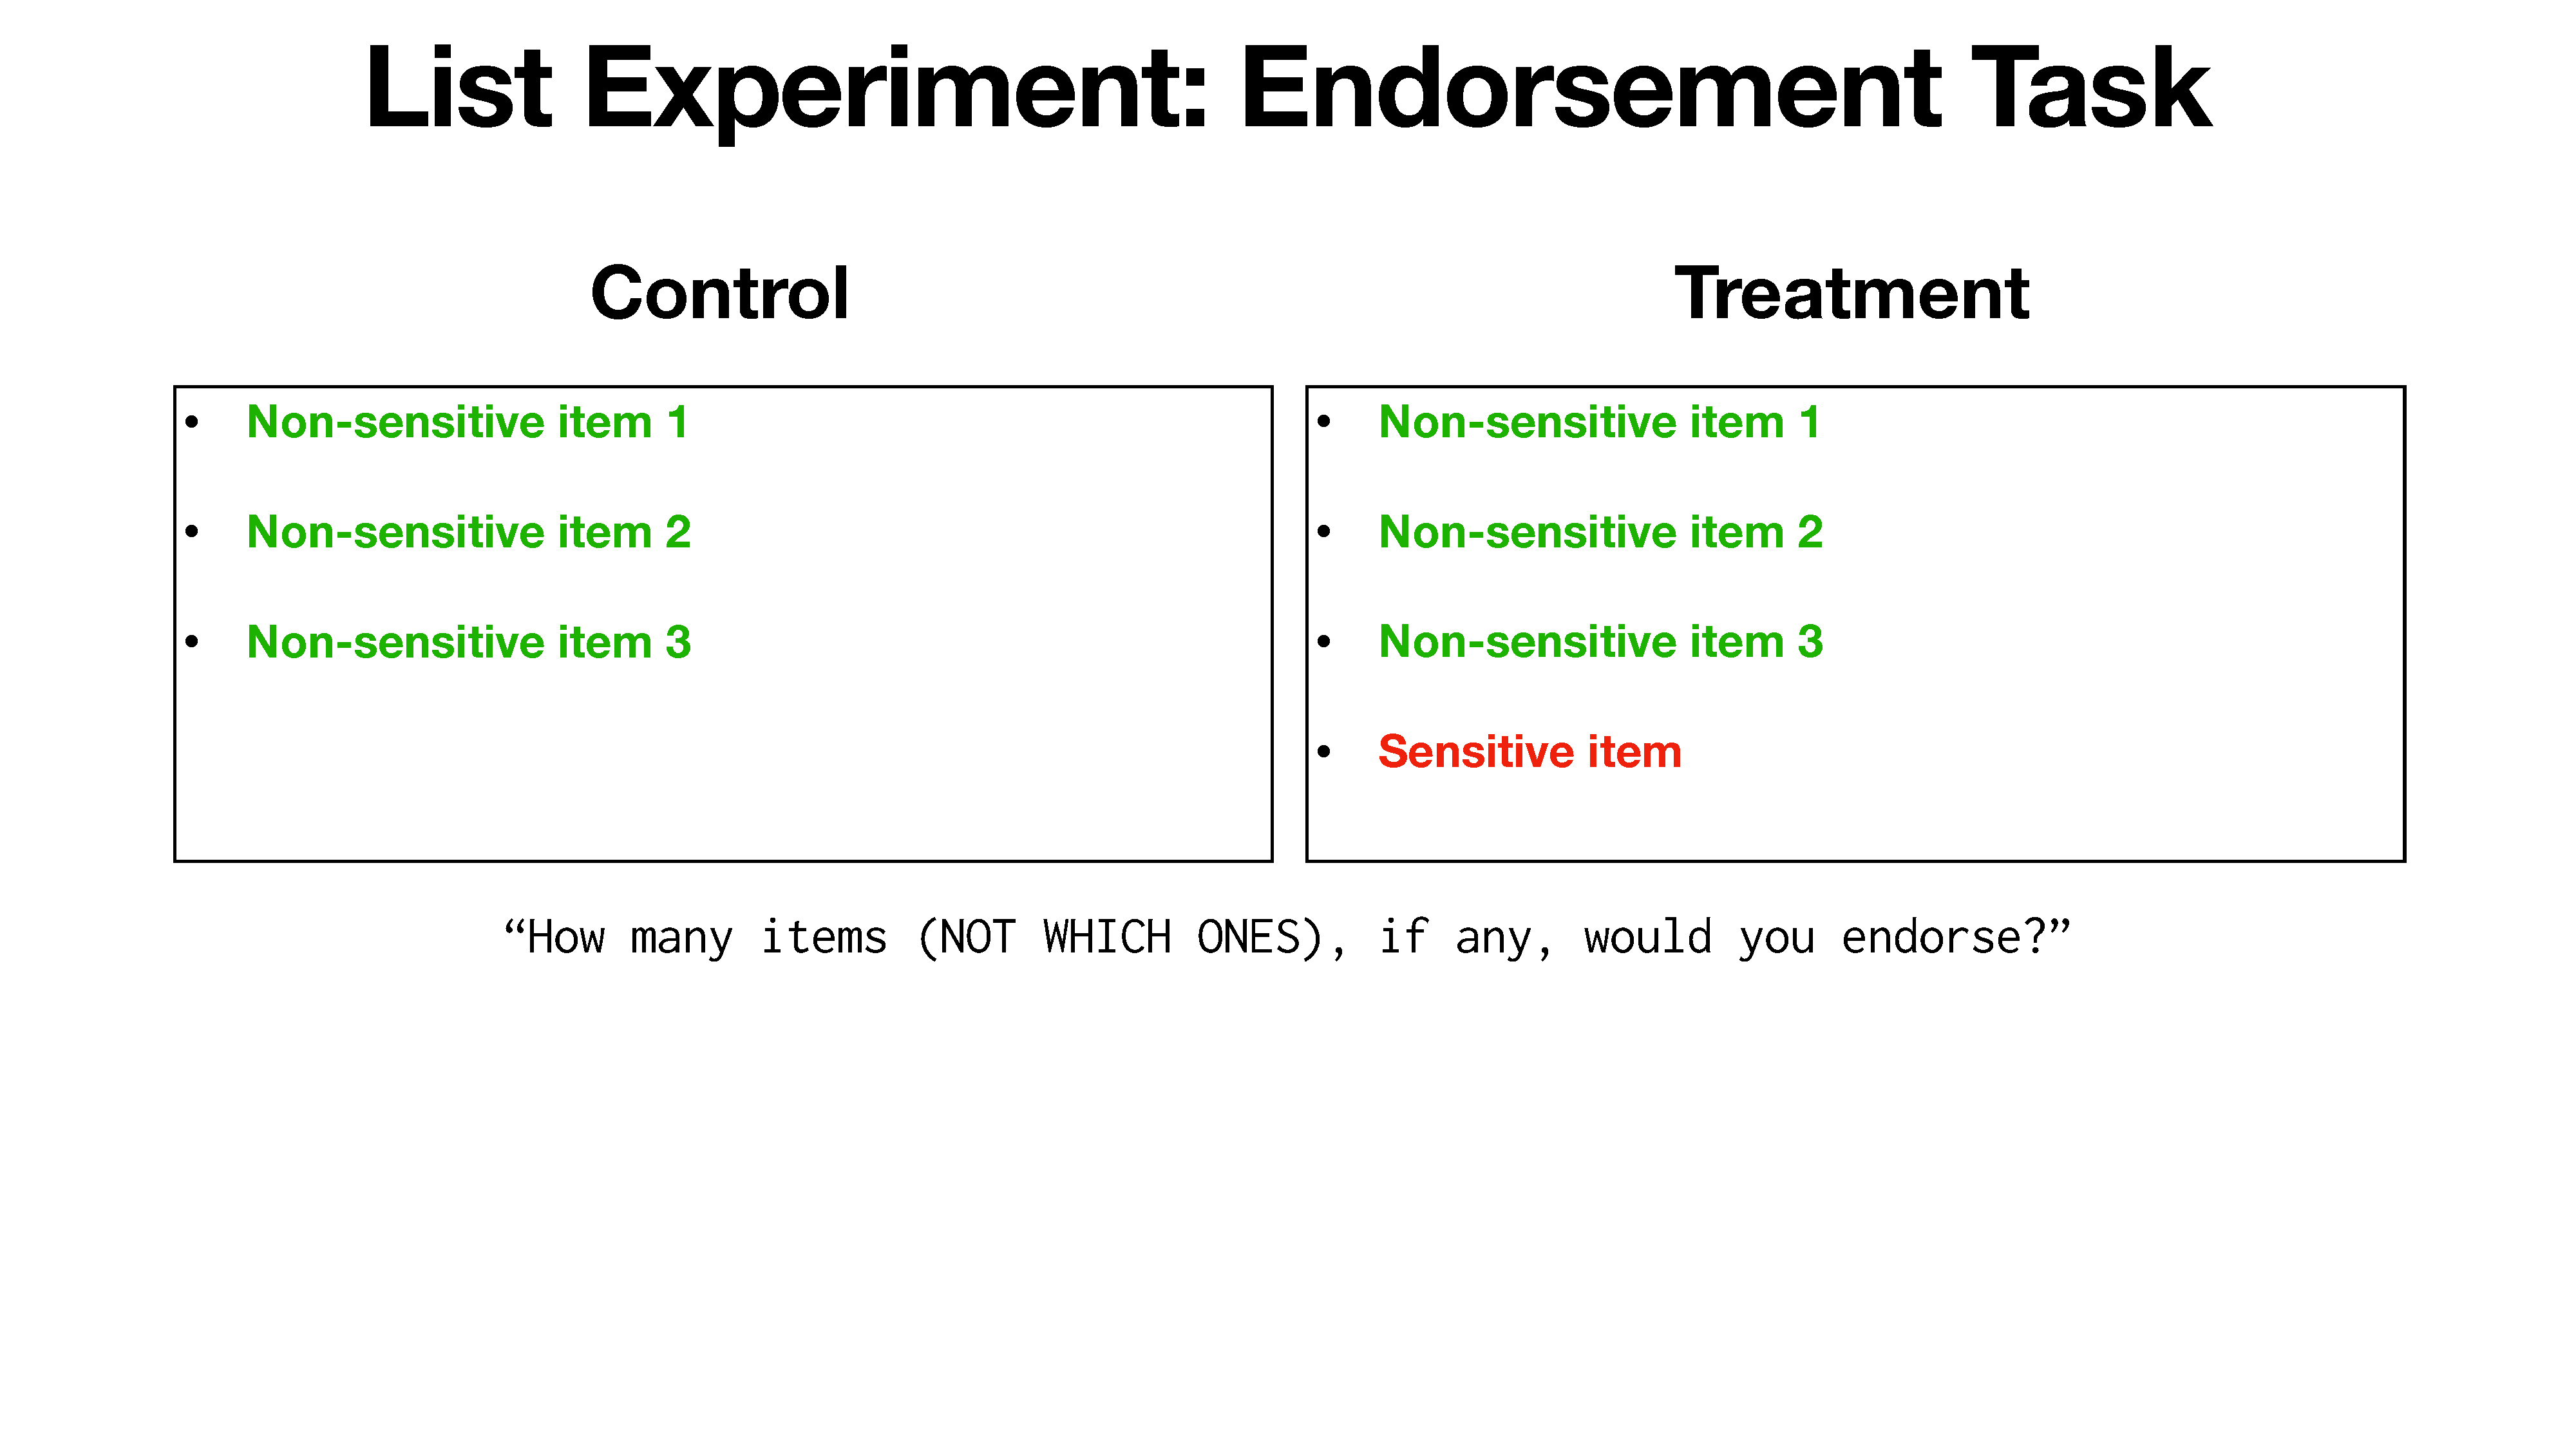
\includegraphics[scale=0.22]{/Users/hectorbahamonde/research/Vote_Selling/LE_1.pdf}
\end{frame}


\miniframesoff
\begin{frame}[plain]
 %\vspace{-0.5cm}
  \centering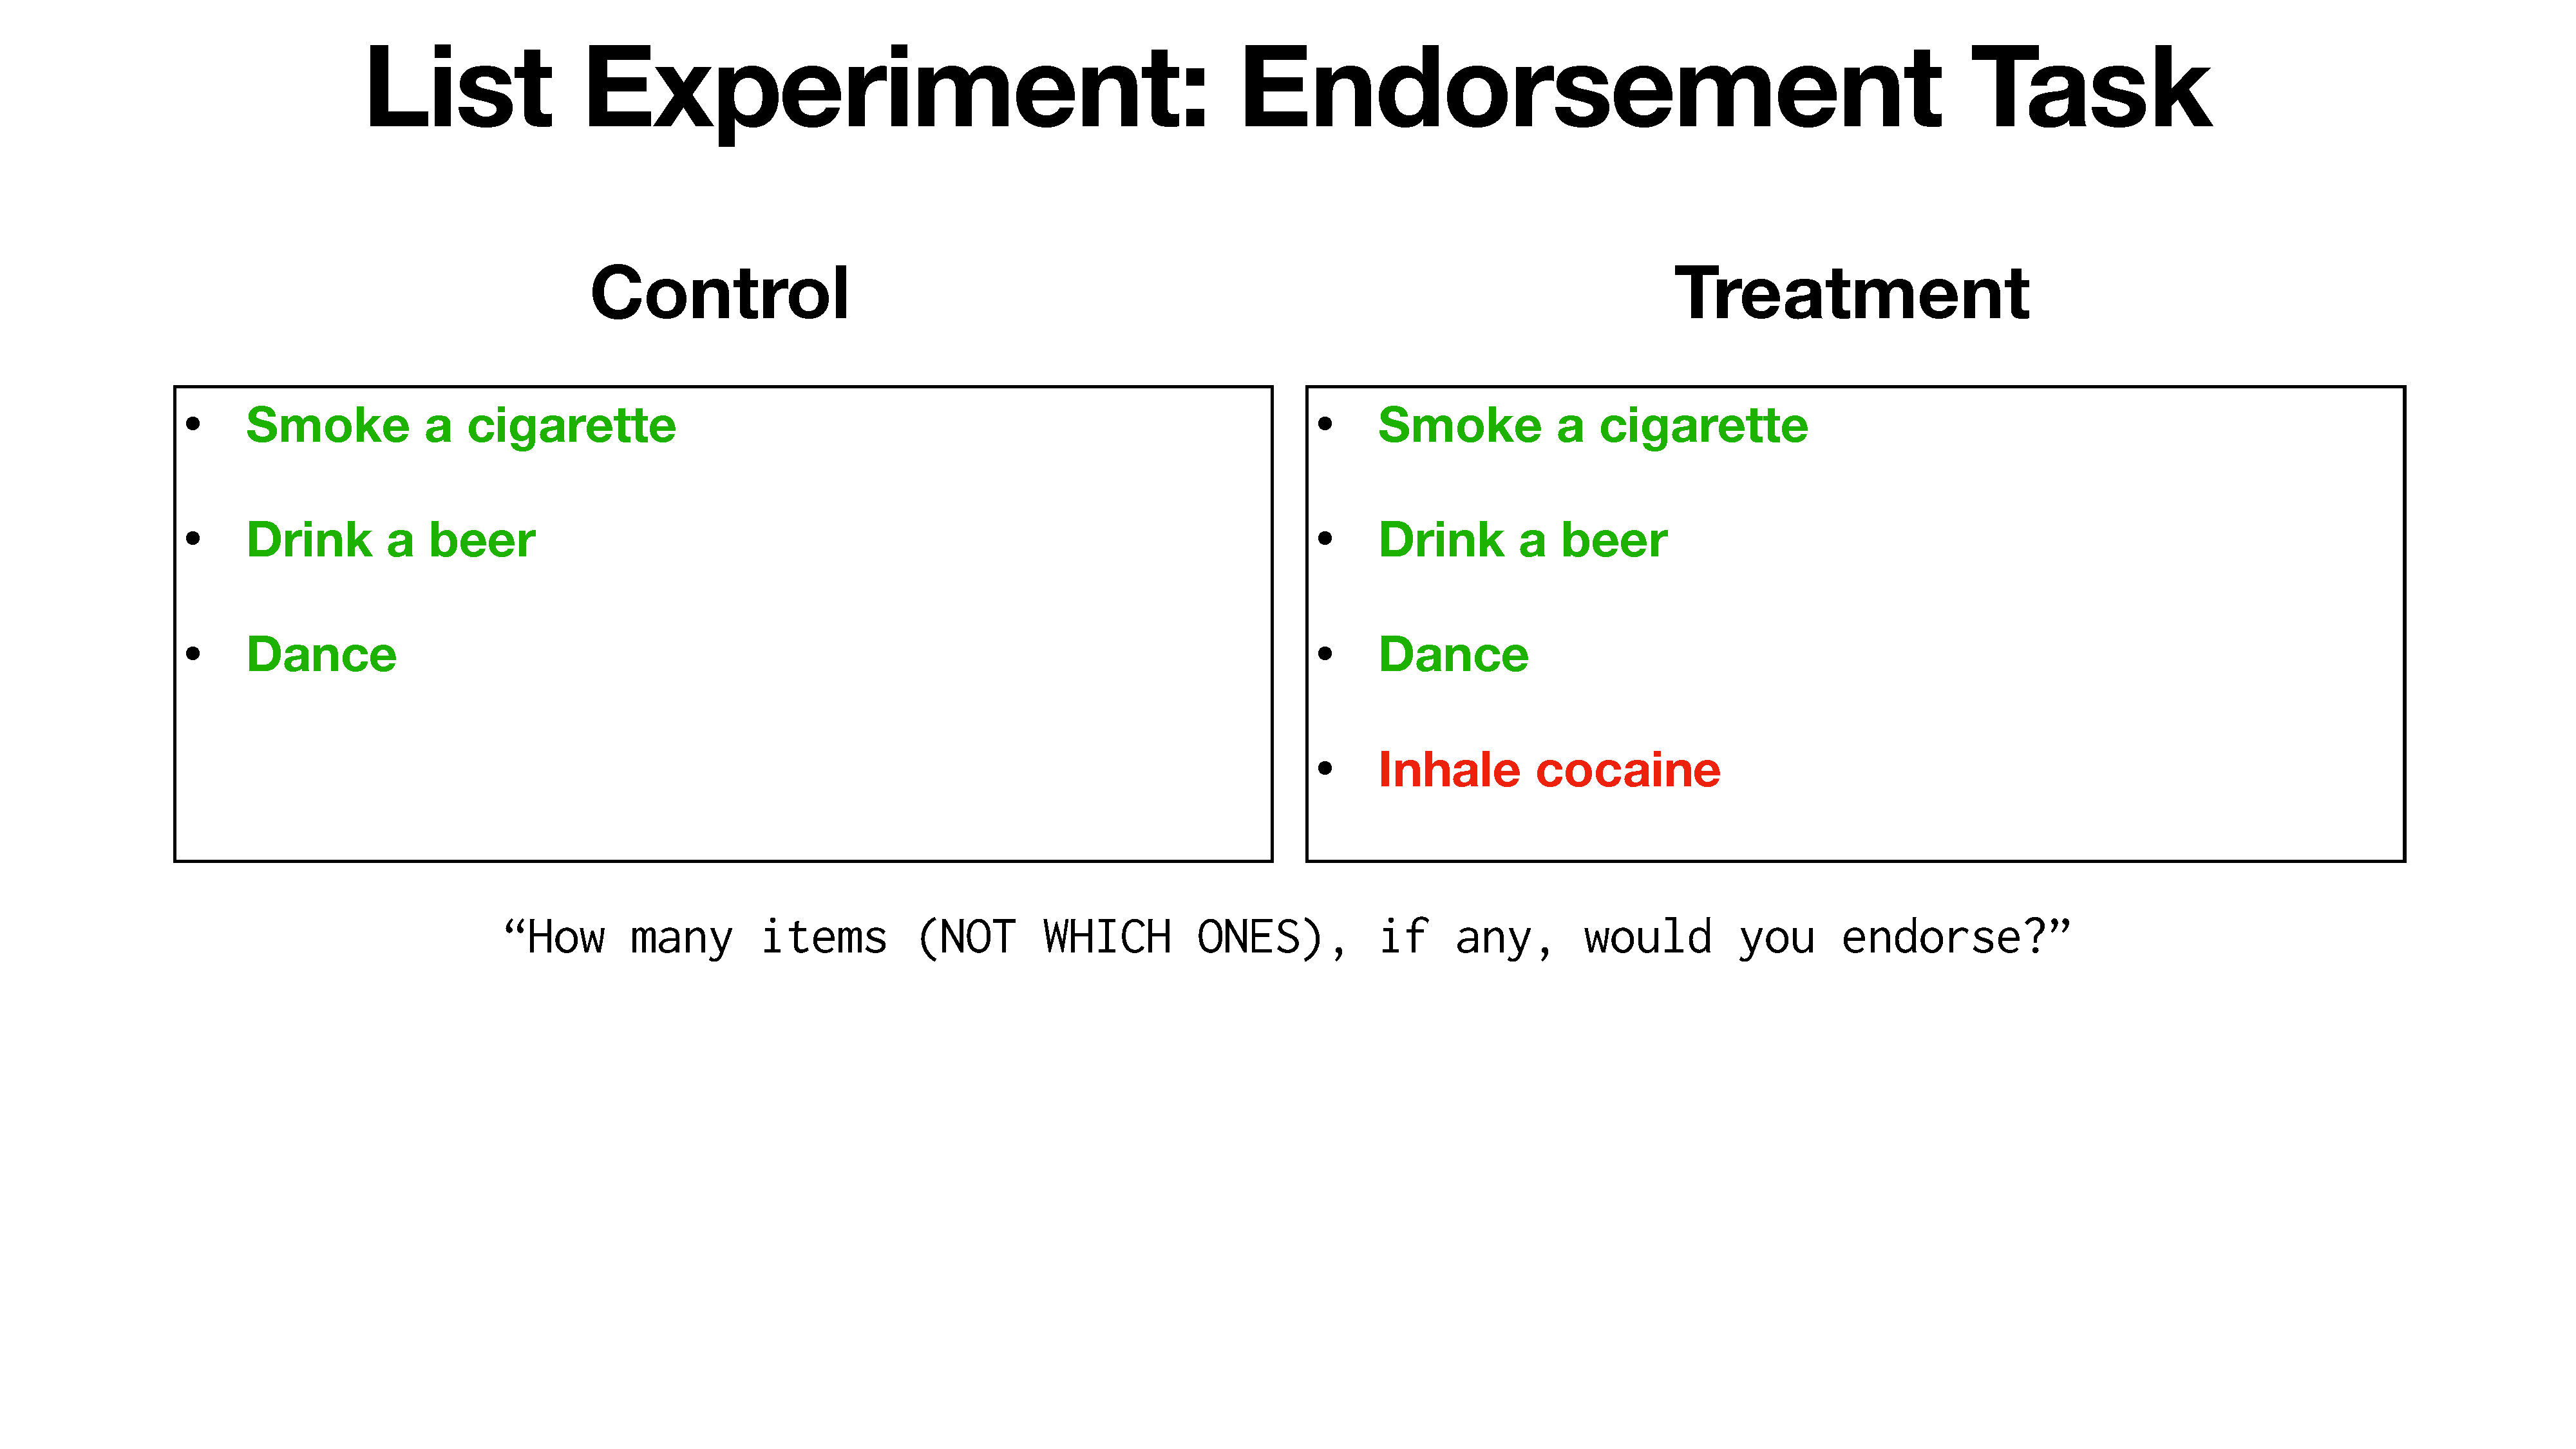
\includegraphics[scale=0.22]{/Users/hectorbahamonde/research/Vote_Selling/LE_2.pdf}
\end{frame}


\miniframesoff
\begin{frame}[plain]
 %\vspace{-0.5cm}
  \centering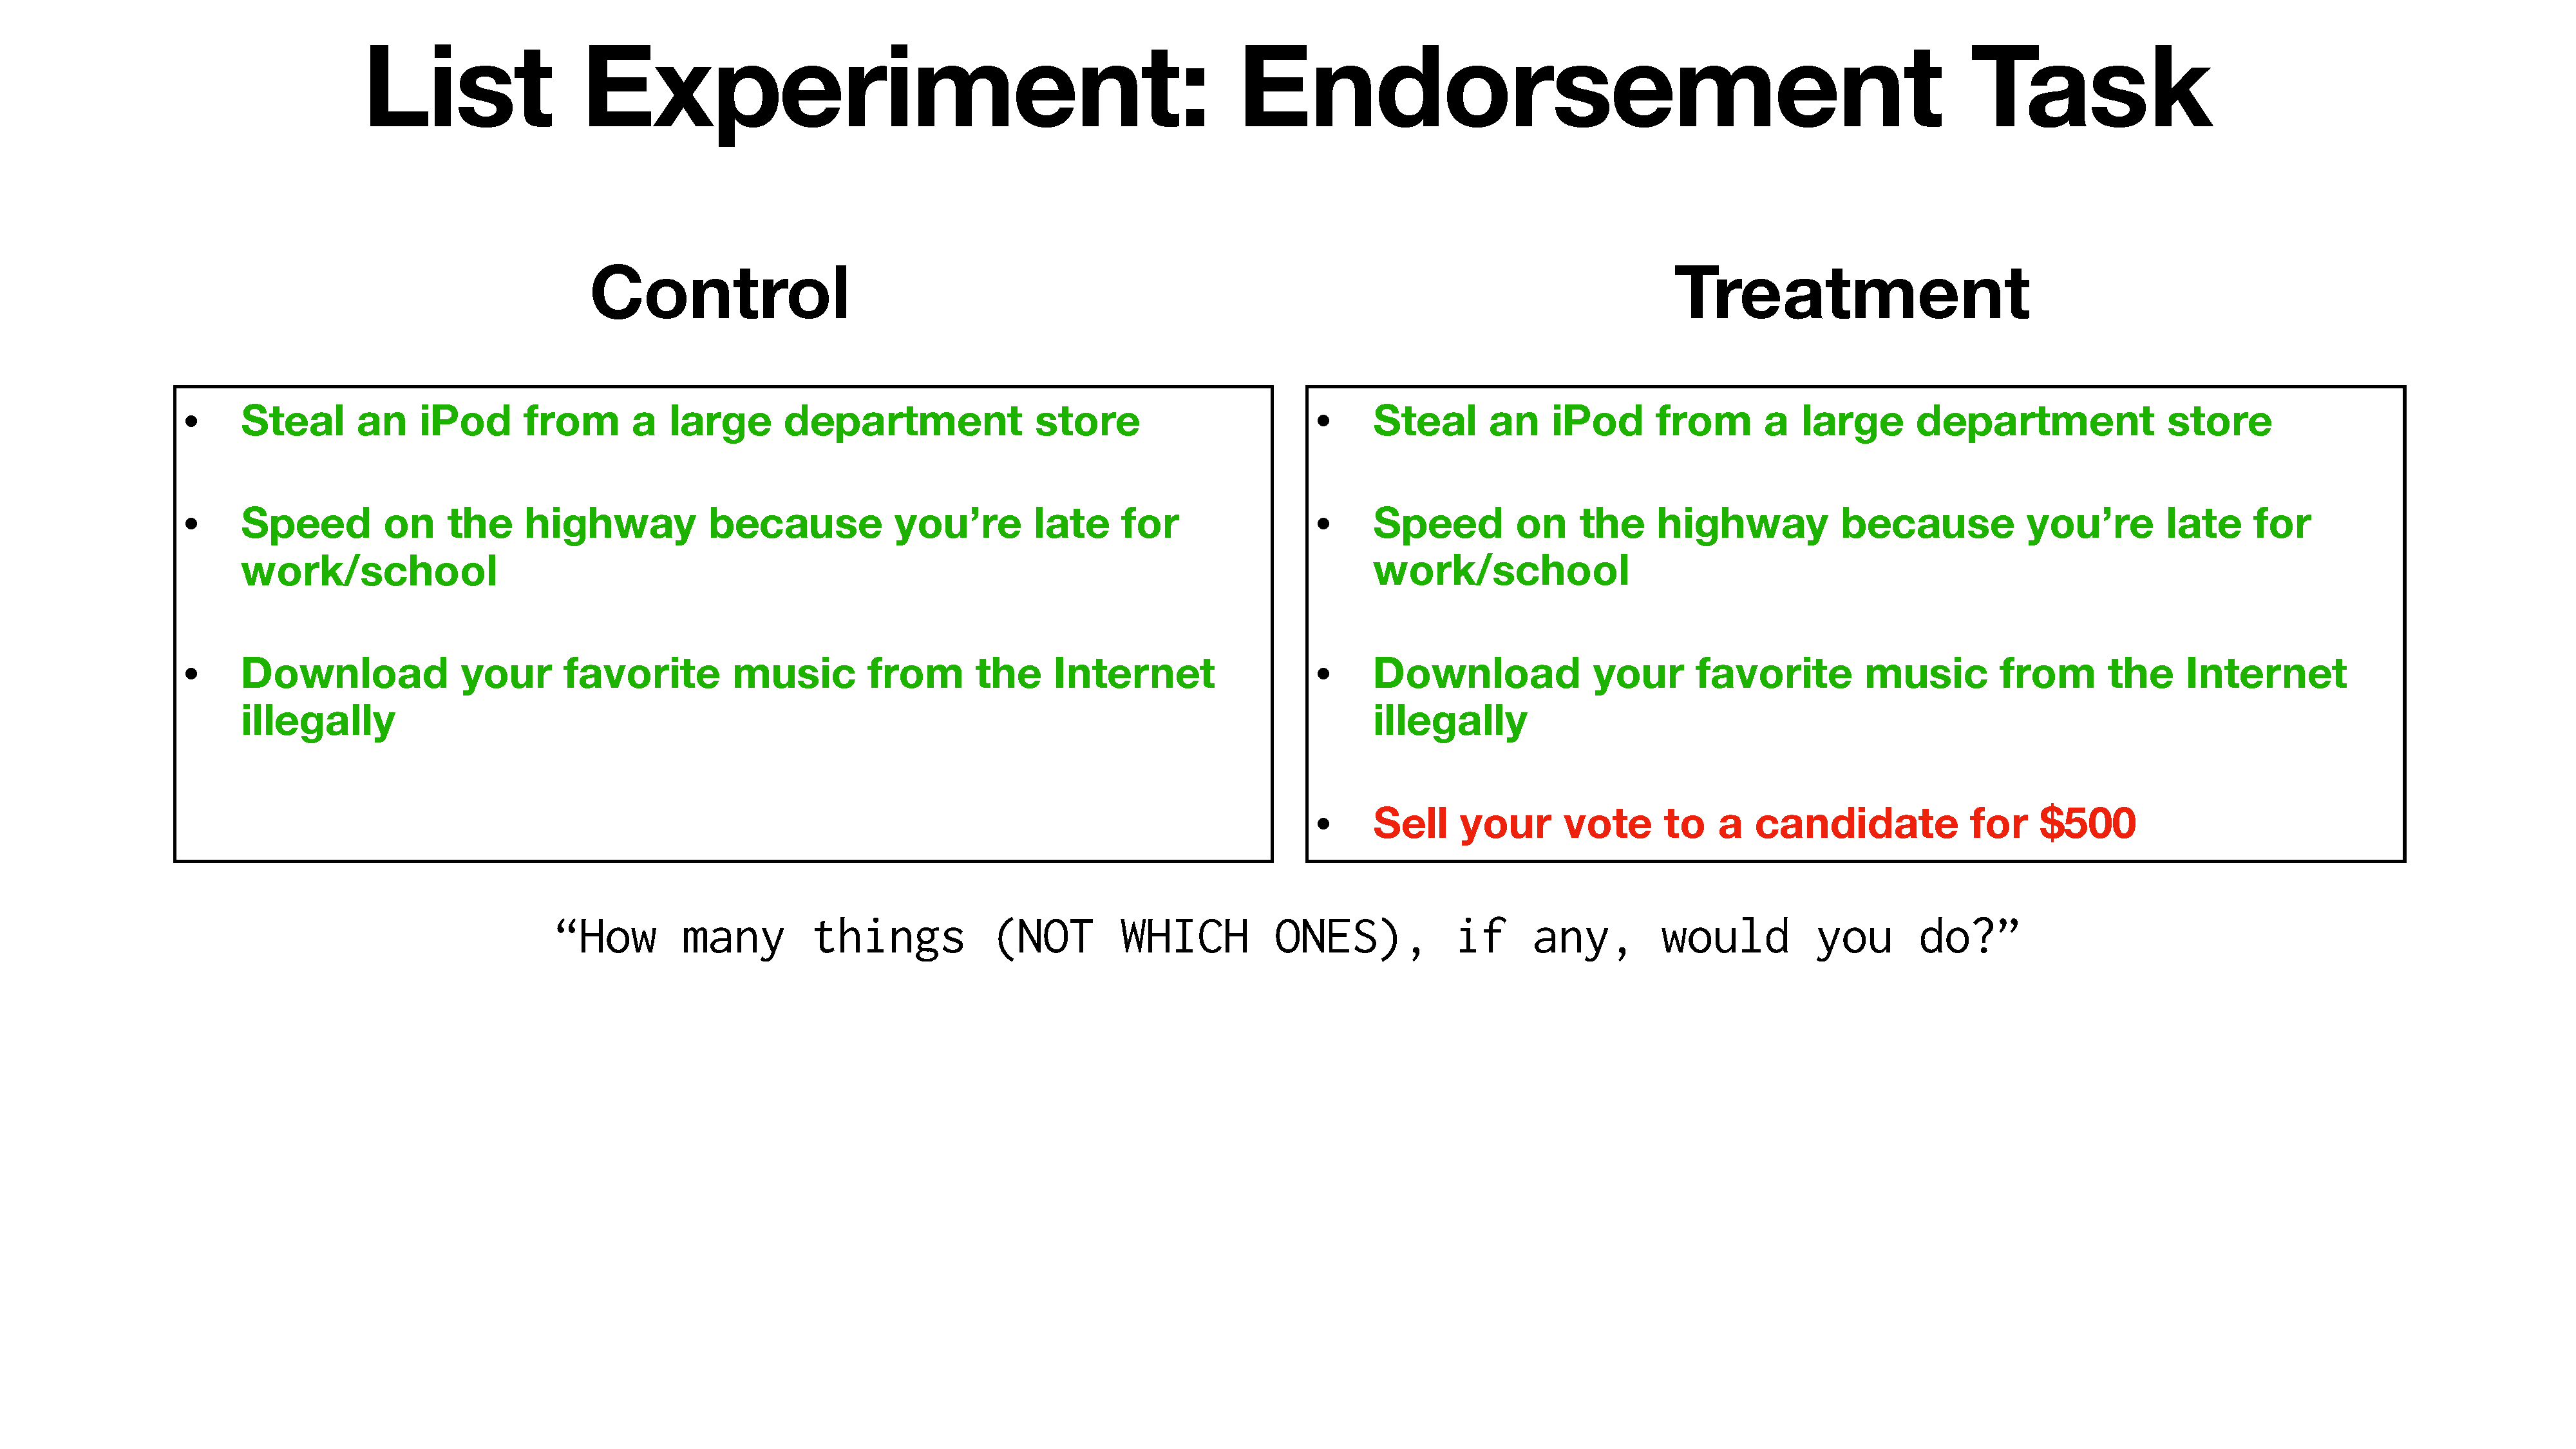
\includegraphics[scale=0.22]{/Users/hectorbahamonde/research/Vote_Selling/LE_3.pdf}
\end{frame}

\miniframeson
\begin{frame}\frametitle{My Experimental Design: Controlling for Ordering Effects}
 %\vspace{-0.5cm}
  \centering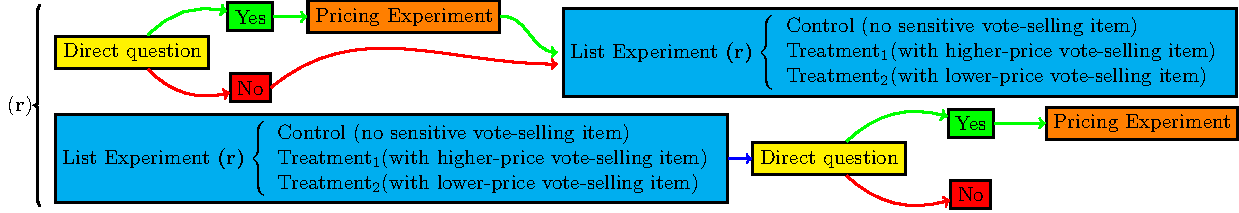
\includegraphics[scale=0.65]{/Users/hectorbahamonde/research/Vote_Selling/Experimental_Flow_Figure.pdf}
\end{frame}





\subsection{Outcome: Count Variable}

\miniframeson
\begin{frame}\frametitle{Dependent Variable}
\begin{minipage}{0.4\textwidth}
    \begin{itemize}
          \item Item count for subject $i$, broken by experimental regime.
          \item Two treatments were administered (``cheap''/``expensive''): they account for possible elasticities.\\{\scriptsize Hard to price a vote.}
    \end{itemize}
\end{minipage}
\begin{minipage}{0.5\textwidth}
\centering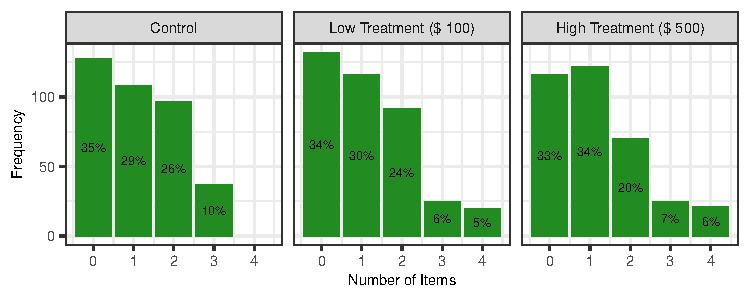
\includegraphics[scale=0.6]{/Users/hectorbahamonde/research/Vote_Selling/figure/barplot:figure:control:treatment-1.pdf}
\end{minipage}
\end{frame}


\subsection{Identification Strategy}

\miniframeson
\begin{frame}\frametitle{Modeling Individual Probabilities of Vote Selling}
    \begin{itemize}
    	\item While list experiments are straightforward, difference in means analyses are:
        \begin{itemize} 
          \item inefficient (wide confidence intervals). 
          \item unable to tell us anything about individual preferences toward vote buying.\pause
        \end{itemize}
        \item {\bf Multivariate approach}: Estimate what we cannot observe (vote selling) using information that we do observe (socio-economic questionnaire).\pause
        	\begin{itemize}
            \item {\bf Poisson-Binomial distribution}: questionnaire is used to build via MLE estimators a profile of subject types ``1'', ``2,'' ``3'' and ``4.''
            \item {\bf Potential outcomes framework}: statistically infer who \emph{would} have answered ``4'' (vote selling).
        			%\begin{enumerate}
        			%	\item Model marginal distribution of the response to control items.
        			%	\item Model the conditional distribution of the response to the sensitive item \emph{given} the response to the control items.
        			%	\item {\tiny Marginalize the conditional expectation of the Poisson–Binomial distribution via maximum likelihood.}
        			%\end{enumerate}
    		\end{itemize}
    \end{itemize}
\end{frame}


\subsection{Results}

\miniframeson
\begin{frame}\frametitle{Individual Results}
\centering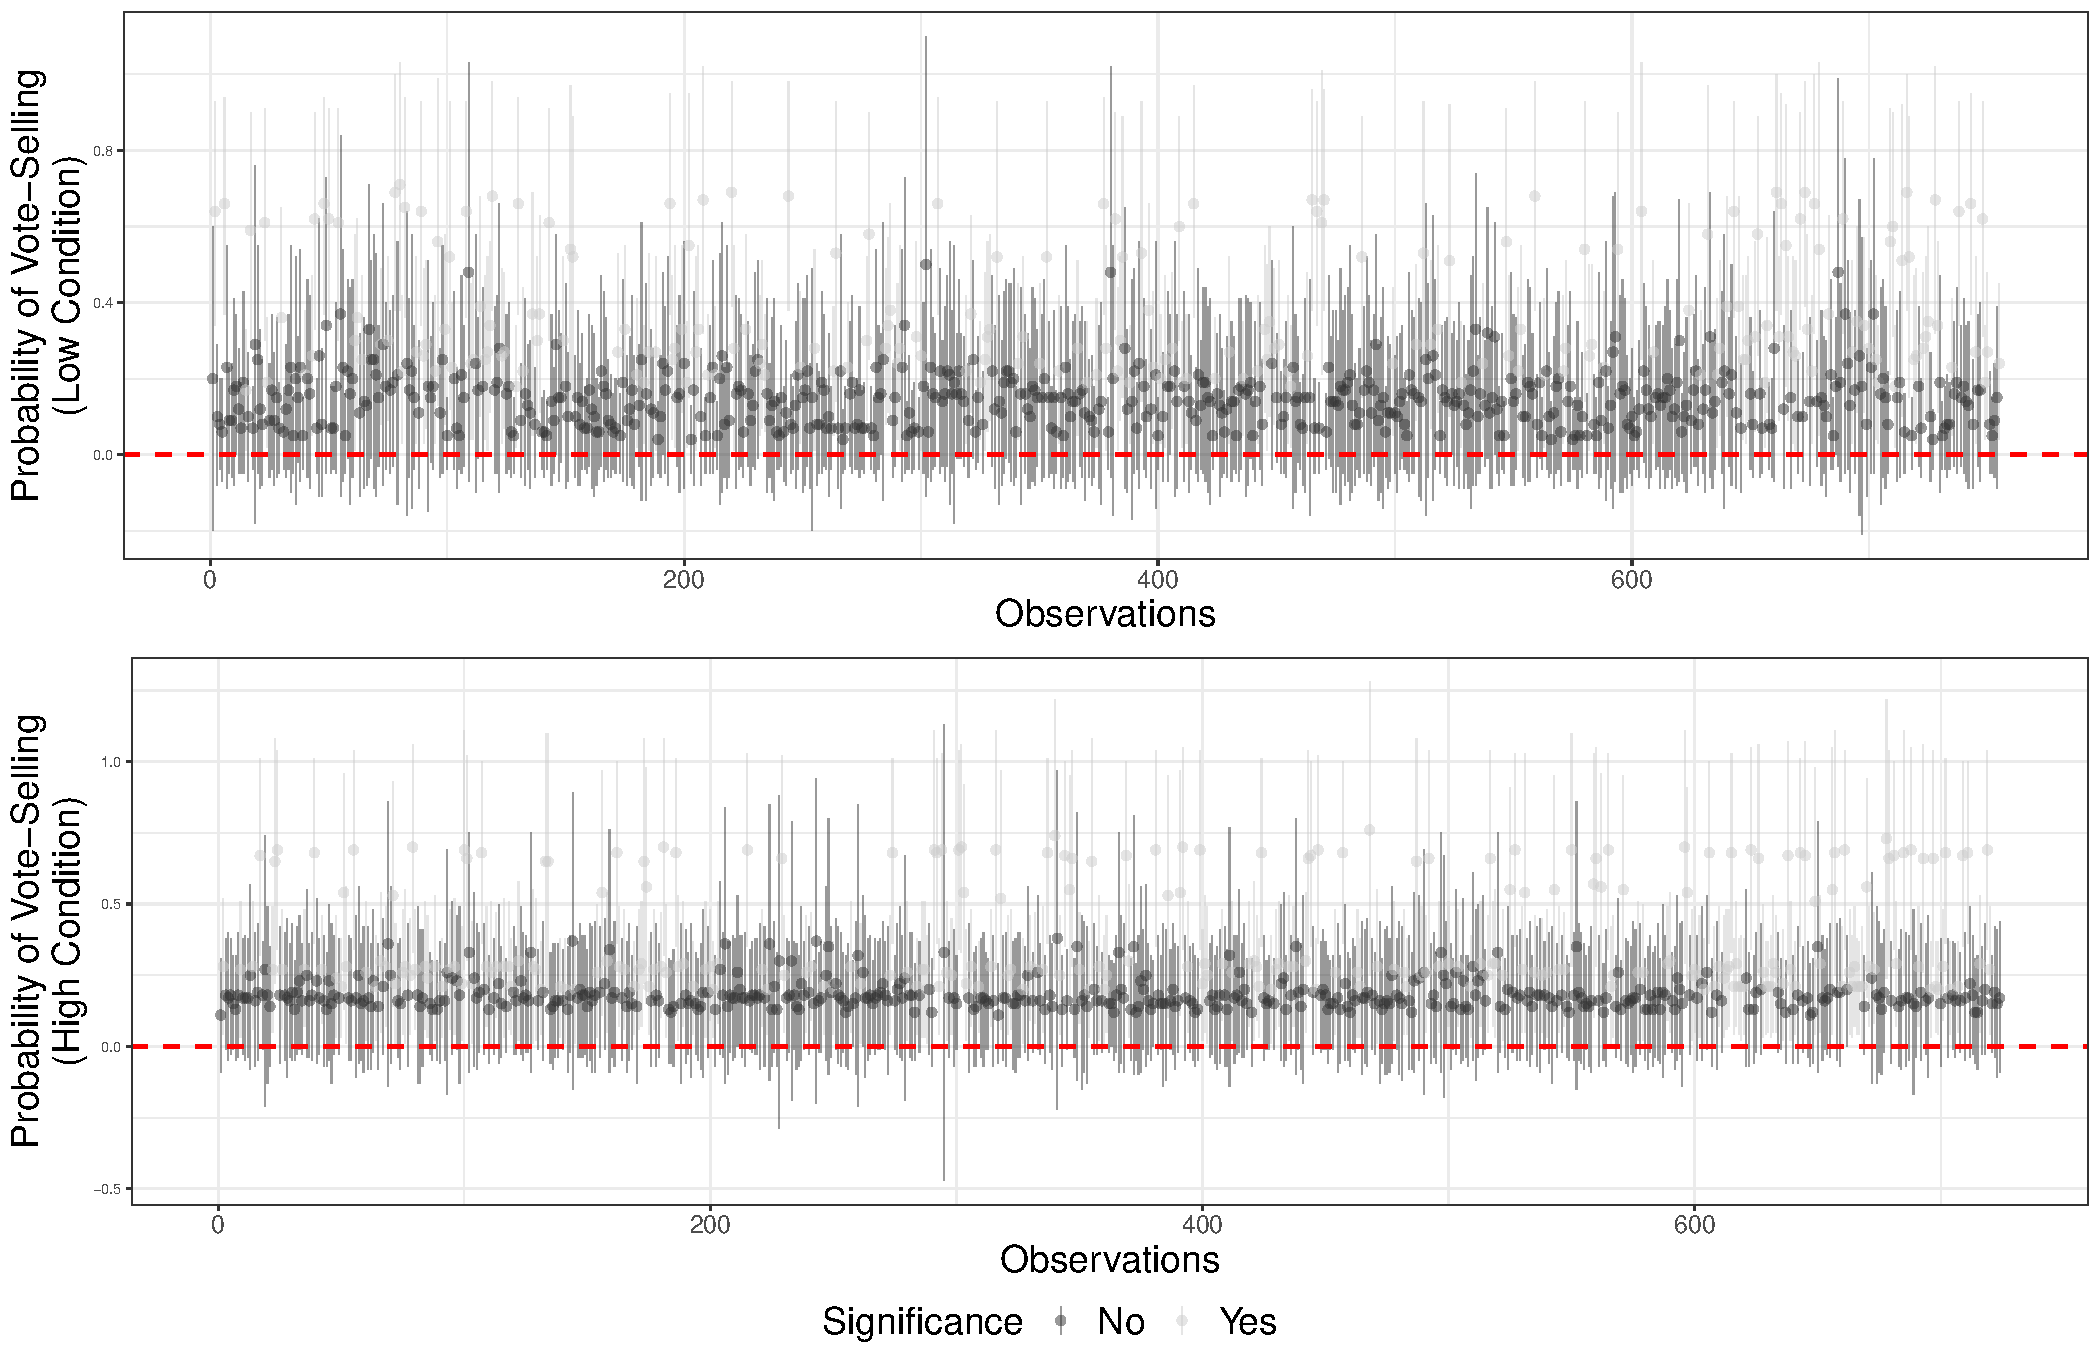
\includegraphics[scale=0.3]{/Users/hectorbahamonde/research/Vote_Selling/figure/list:analysis:individual:predictions:plot-1.pdf}
\end{frame}

\miniframeson
\begin{frame}\frametitle{Results: Who wants to sell and who's lying?}
\begin{minipage}{0.4\textwidth}
    \begin{itemize}
          \item Dif in means: inefficient.
          \item List experiment: 25\% would be willing to sell their vote.
          \item Only 18\% sells when directly asked.
          \item 7\% lied (due to social desirability bias).
    \end{itemize}
\end{minipage}
\begin{minipage}{0.5\textwidth}
\centering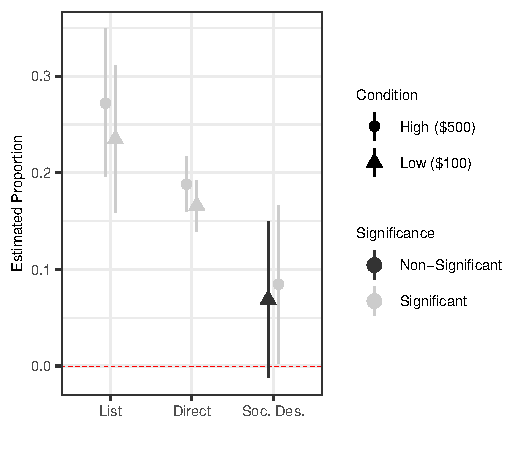
\includegraphics[scale=0.65]{/Users/hectorbahamonde/research/Vote_Selling/figure/list:analysis:social:desirability:plot-1.pdf}
\end{minipage}
\end{frame}







\miniframeson
\begin{frame}\frametitle{Price Test: In USD   \$1 Increments}
\begin{minipage}{0.45\textwidth}
\centering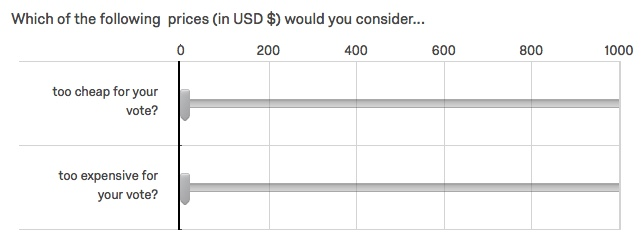
\includegraphics[scale=0.3]{/Users/hectorbahamonde/research/Vote_Selling/pricing_experiment.jpeg}
\end{minipage}
\begin{minipage}{0.5\textwidth}
\centering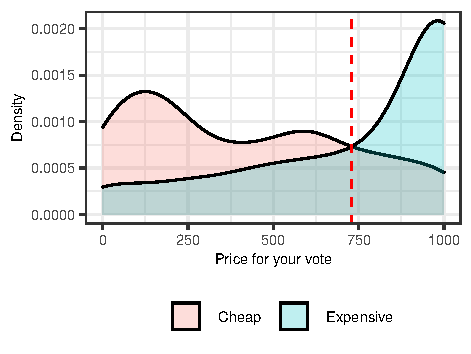
\includegraphics[scale=0.7]{/Users/hectorbahamonde/research/Vote_Selling/price_plot.pdf}
\end{minipage}
\end{frame}


\miniframeson
\begin{frame}\frametitle{Profiling Vote Sellers}
\centering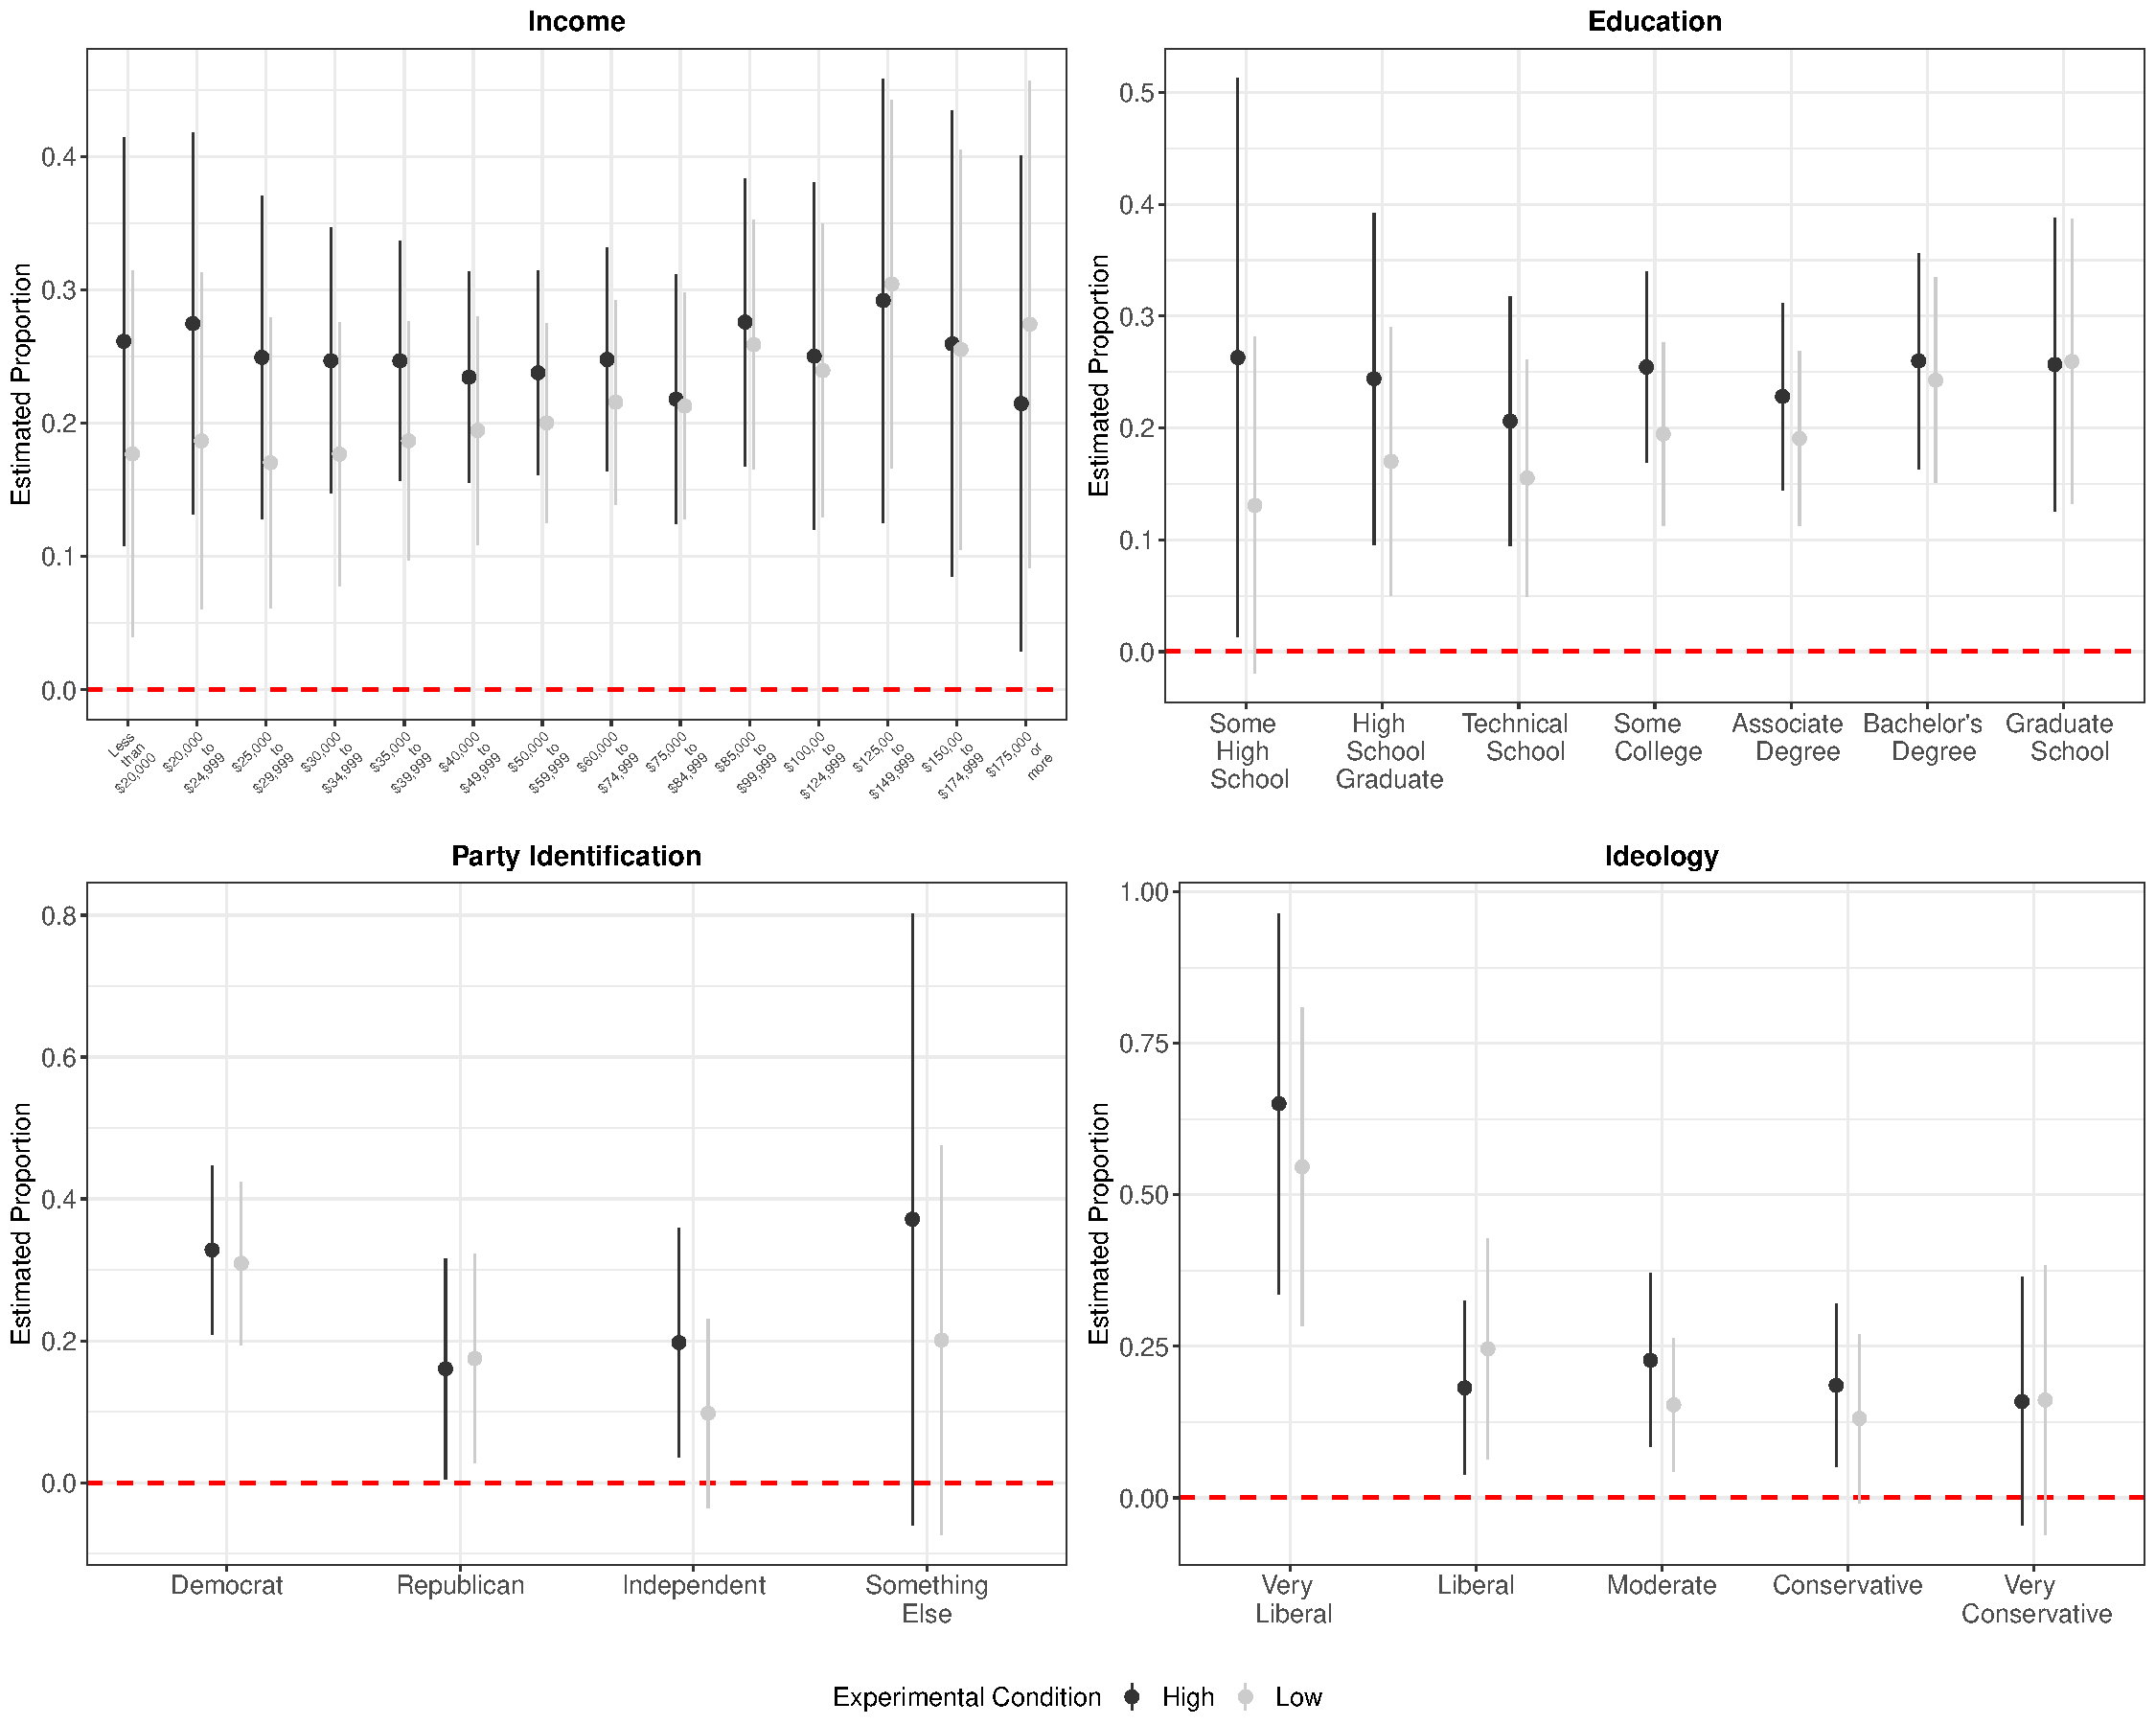
\includegraphics[scale=0.2]{/Users/hectorbahamonde/research/Vote_Selling/figure/predictions:independent:variables:plot-1.pdf}
\end{frame}


\section{Discussion}

\subsection{Summary}

\miniframeson
\begin{frame}\frametitle{What this Talk Was About: Main Findings}
    \begin{enumerate}
      \item Descriptive paper: \emph{why} and \emph{how} were left for future iterations.
      \item Least-likely case design.
      \item Biases: \emph{selection} and \emph{social desirability}.
      \item {\bf Findings}.\pause
        \begin{itemize}
            \item Approximately 25\% of voters in the U.S. would sell their vote.
            \item They would sell it for a minimum payment of \$418. 
            \item Democrats and Liberals are more likely to sell (\emph{why}?).
            \item Education or income levels do not seem to impact the likelihood of vote selling.
        \end{itemize}
   \end{enumerate}
\end{frame}


\subsection{Future Avenues of Research}

\miniframeson
\begin{frame}\frametitle{What's Ahead}
{\bf Future research}:
        \begin{enumerate}
          \item \emph{Paper}(s) y experimento(s) junto a Andrea C\'anales: econom\'ia experimental.
          \item \emph{Paper} junto a Crist\'obal Qui\~ninao usando misma base de datos, pero con un \emph{conjoint experiment}. Uso machine learning para subclasificar \emph{vote-sellers}.
          \item Furura expansi\'on de este experimento via un \emph{Fondecyt}, pero usando metodo comparado (incluir otros paises, por lo pronto, Chile).
          \item {\bf Otros?}
        \end{enumerate}

\end{frame}


\miniframesoff
\begin{frame}[plain,c, label=thank_you]
\begin{center}
\Huge{Gracias}\\
\vspace{1cm} \texttt{www.Hector{\color{black!30!green}{\bf Bahamonde}}.com}
\end{center}
\vspace{1cm}
\end{frame}


\section{Appendix}

\miniframesoff
\begin{frame}\frametitle{Priming Subjects before the Study}
\centering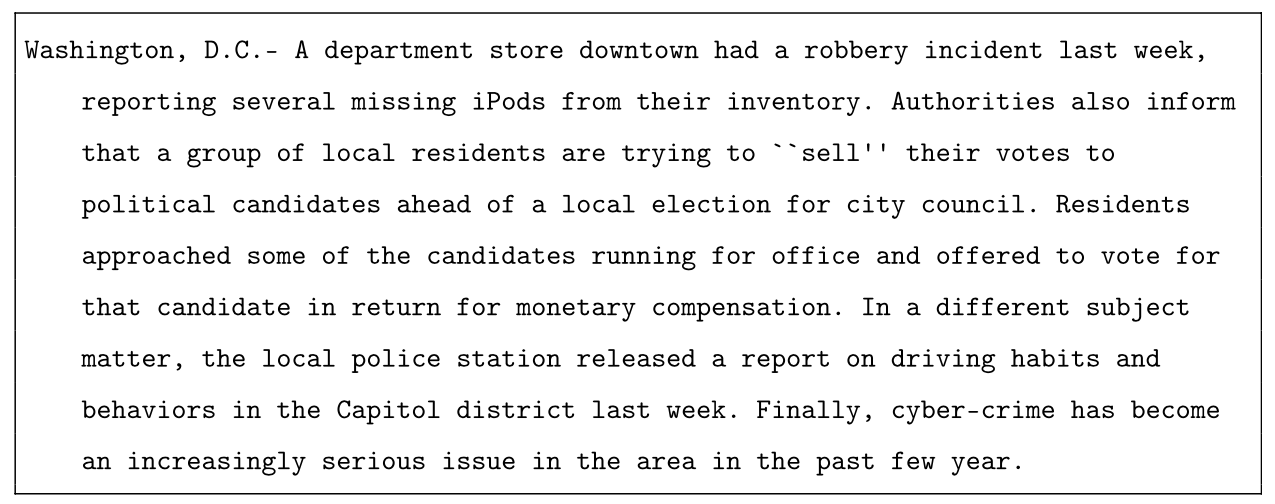
\includegraphics[scale=0.3]{/Users/hectorbahamonde/research/Vote_Selling/Appendix_1.png}
\end{frame}

\miniframesoff
\begin{frame}\frametitle{Distractor Paragraph: Direct Question (I)}
All subjects read the next paragraph, and then all answered the direct question
\centering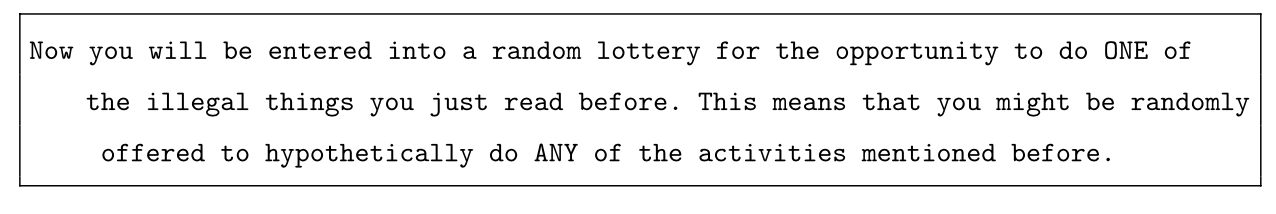
\includegraphics[scale=0.3]{/Users/hectorbahamonde/research/Vote_Selling/Appendix_2.png}
\end{frame}


\miniframesoff
\begin{frame}\frametitle{Distractor Paragraph: Direct Question (II)}
\centering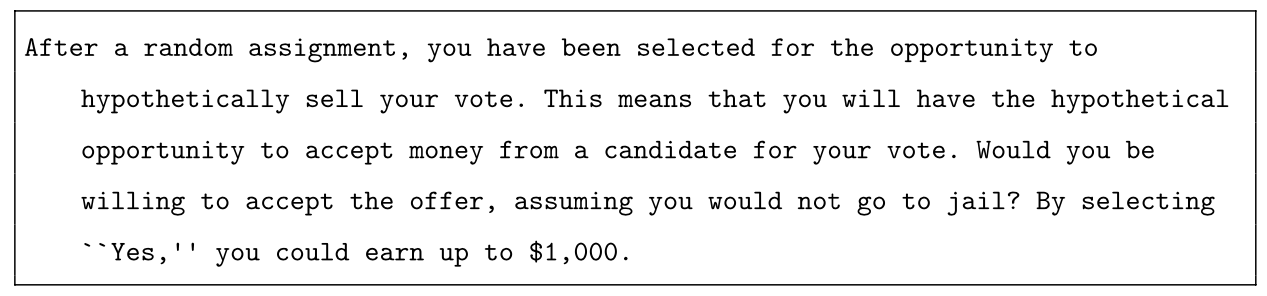
\includegraphics[scale=0.3]{/Users/hectorbahamonde/research/Vote_Selling/Appendix_3.png}
\end{frame}


\end{document}


